\documentclass[11pt,a4paper]{article} % Mandatory
\usepackage[T1]{fontenc} % Support for fonts with æøå and other foreign characters.
\usepackage[utf8]{inputenc} % Support for UTF-8 encoded input documents
\usepackage{fullpage}
\usepackage{graphicx} % Support for including graphics as png, gif, and jpeg
\usepackage{amssymb} % Support for alterantive symbols
\usepackage{amsmath} % Support for mathematical symbols
\usepackage{listliketab} % Support for tabulated lists
\usepackage{enumitem} % Support for indented description items and more
\usepackage[parfill]{parskip} % Support for American style paragraphs
\usepackage{color} % Support for colored text
\usepackage{listings} % Support for code listings
\usepackage{nameref} % Enables refernces to names.
\usepackage{makeidx} % For creating indexes
\usepackage{hyperref} % For using URLs
\usepackage{xspace} % For adding a space only when necessary.
\usepackage{todonotes} % For adding TODOs
\usepackage{titling} % For modifying subtitle

\newcommand{\subtitle}[1]{%
  \posttitle{%
    \par\end{center}
    \begin{center}\large#1\end{center}
    \vskip2em}%
}


\title{Fault Protection for Space Missions}
\subtitle{02228 - Fault-Tolerant Systems\\
Autumn 2013}
\author{
  Cosmin Stefan-Dobrin\\
  Technical University of Denmark\\
  \texttt{s121038}
  \and
  Rafaela Voiculescu\\
  Technical University of Denmark\\
  \texttt{s120931}
}
\date{}

\begin{document}
\begin{titlepage}
\maketitle 
\thispagestyle{empty}
\vfill
\begin{abstract}
\textit{Space has been a topic of high interest in the past century and the
space exploration missions have aimed to help new discoveries. The spacecrafts
used for this purpose have been designed for the unknown, high-risk nature of
the missions and, thus, fault protection has been an important necessity. This
paper offers a brief analysis of general approaches and specific implementations
for fault management architectures used in space exploration missions. }
\end{abstract}
\end{titlepage}
\newpage

\tableofcontents


\section{Introduction}
For more than 50 years the human kind has been sending ships into the outer
space in order to look for answers to centuries-old questions about what is
beyond our atmosphere. And we have managed to explore and understand more and
more of our Solar System and the space beyond. The successful missions have been
the result of the reliable architectural design, implementation and testing done
by the engineers working on them.

The extremely high costs, in both money and time, and the high risks of such
missions require an extremely high level of reliability that can guarantee a
very high chance of success. Thus, fault protection of the systems involved in
these missions is of utter importance.

Spacecrafts are extremely complex and their design is usually very specific to
the particular mission objective. Furthermore, space missions are meant to have
a duration of months or years and sustain operation in extreme environment and
under harsh conditions. This, in addition to financial and temporal limitations,
make the design of fault protection mechanisms a challenging task for the
engineers. When taking into consideration the deep space exploration missions
(i.e missions meant to last for multiple years and have the purpose of exploring
the Solar System and beyond), an even higher level of reliability is required
and various techniques to assure fault prevention, detection, containment and
recovery need to be employed to assure mission success.

This paper aims to take a look into the fault protection approaches used in the
spacecrafts domain, with a particular focus on deep space explorations missions.
A general look at the characteristics of such missions is first taken, followed
by a brief introduction to the general approaches followed when designing and
implementing fault protection for spacecrafts. Then, a series of previous space
missions (both successful and unsuccessful) are analyzed, with a focus on the
fault management.

\section{Requirements for spacecrafts}
\section{Generic Spaceship Architecture}
One of the most important characteristics of this domain is that spacecraft
missions have extremely diverse purpose, so the design of each is specific and
unique. The spacecrafts that go outside Earth's atmosphere vary from simple ones
(e.g. satellites) to very complicated ones (e.g. deep-space missions). However,
the principles on which their designs are based are common. Virtually all the
spacecrafts have similar requirements regarding aspects such as power,
telecommunications, propulsion etc. and share a general structural construction.
Thus, in order to aid the understanding of the Fault-Tolerant approaches used
for space missions, a generic architecture for spacecrafts is briefly described.

Typically, spaceships have an architecture that contains, at minimum, 5
subsystems\cite{ft-space-avionics}. These are \textit{propulsion},
\textit{communications}, \textit{power}, \textit{attitude control} and
\textit{command \& control}, as seen in Figure~\ref{fig:generic_structure}.

\begin{description}
  \item[Propulsion] This subsystem is in charge of accelerating and stabilizing
  the ship and controlling its orientation. Multiple methods can be used for
  propulsion, but the most common ones are gas\footnote{Chemical or pressurized
  gas is forced at a high speed through a nozzle. This is still the most common
  method.} or electric\footnote{Commonly ion thrusters or Hall effect thrusters
  are used.} based.
  \item[Communication] This subsystem handles the communication between the
  spaceship and the Earth control center. The spacecraft employs transmitters
  and receivers to send and receive messages which travel through space as radio
  waves. The communication going from a satellite to ground is called downlink
  and the one going from ground to a satellite is called uplink. Unlike the
  other modules, the Communications subsystem interfaces not only with
  components on the ship, but also with external entities.
  \item[Power] All the component of a spacrafts Spacecraft require electrical
  power for powering the various functions. This subsytem is in charge of the
  generation, storage and distribution of electrical energy in the spaceship.
  Various generation methods are employed\footnote{ For ships near the Sun,
  solar panels are frequently used to generate electrical power. In more distant
  locations, for example Jupiter, might employ a Radioisotope Thermoelectric
  Generator (RTG) to generate electrical power.}, the most common one involving
  solar cells. The power is passed through a power distribution unit over an
  electrical bus to other spacecraft components. Batteries are used to provide
  electrical power during periods when primary power is not available.
  \item[Attitude Control] This subsystem handles the correct orientation and
  stability of the spacecraft by responding to external torques and forces. Its
  main components are sensors and actuators and uses specialized algorithms for
  control.
  \item[Command/Control] All the aspects related to the spaceship's control are
  handled by this subsystem. Its main tasks include: receives commands from
  the communications subsystem; validates, decodes and distributes the commands
  to the appropriate spacecraft components; receives internal and scientific
  data from the other spacecraft subsystems and components and packages the data
  for storage on a data recorder or transmission to the ground. Also, this
  subsystem is in charge of system health-monitoring and recovery from failures.
\end{description}

\begin{figure}[htb]
\begin{center}
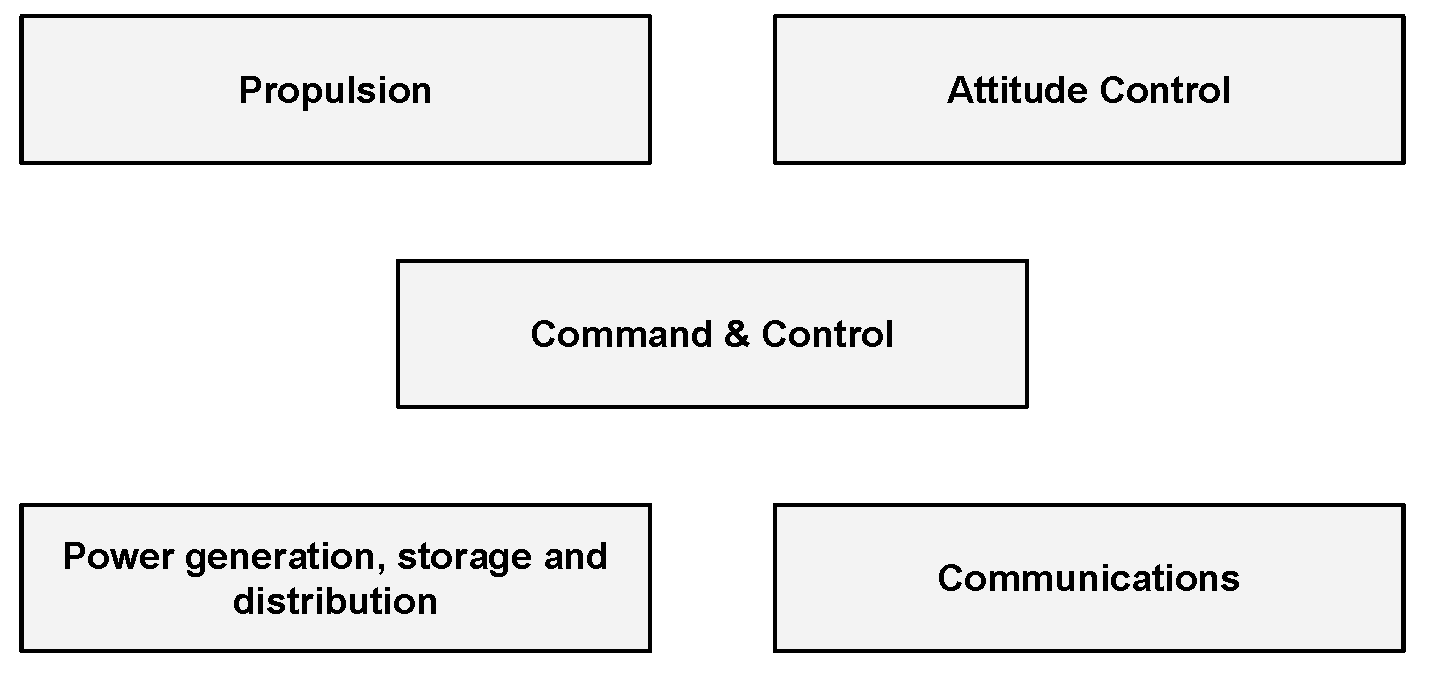
\includegraphics[width=0.92\textwidth]{img/generic_structure.pdf}
\caption{Components of Generic Spacecraft}
\label{fig:generic_structure}
\end{center}
\end{figure}

\section{Approach to fault tolerance in spacecrafts}

The characteristics of space exploration missions have always required
innovative fault management (FM) strategies\footnote{The term \textit{Fault
Management} is often used interchangeably with the term \textit{Fault
Protection} in NASA documentation.} in order to achieve mission success.
The used FM strategies and implementations vary significantly from mission to
mission, but there are a set of general characteristics that influence the
design of the FM. Engineers from NASA have been working on a Fault Management
Handbook with the purpose of being \textit{`a guidance document to provide
guidelines and recommendations for defining, developing, analyzing, evaluating,
testing, and operating the Fault Management (FM) element of flight
systems`}\cite{nasa-fm-handbook}.
 
According to \cite{nasa-fm-handbook}, a space missions FM engineer has the role
of analysing mission attributes and characteristics and defining FM
requirements, as well as developing hardware and software architectures that
provide fault protection and assure the success of missions. This process is
ilustrated in Figure~\ref{fig:fm_design}.

\begin{figure}[htb] 
	\begin{center}
	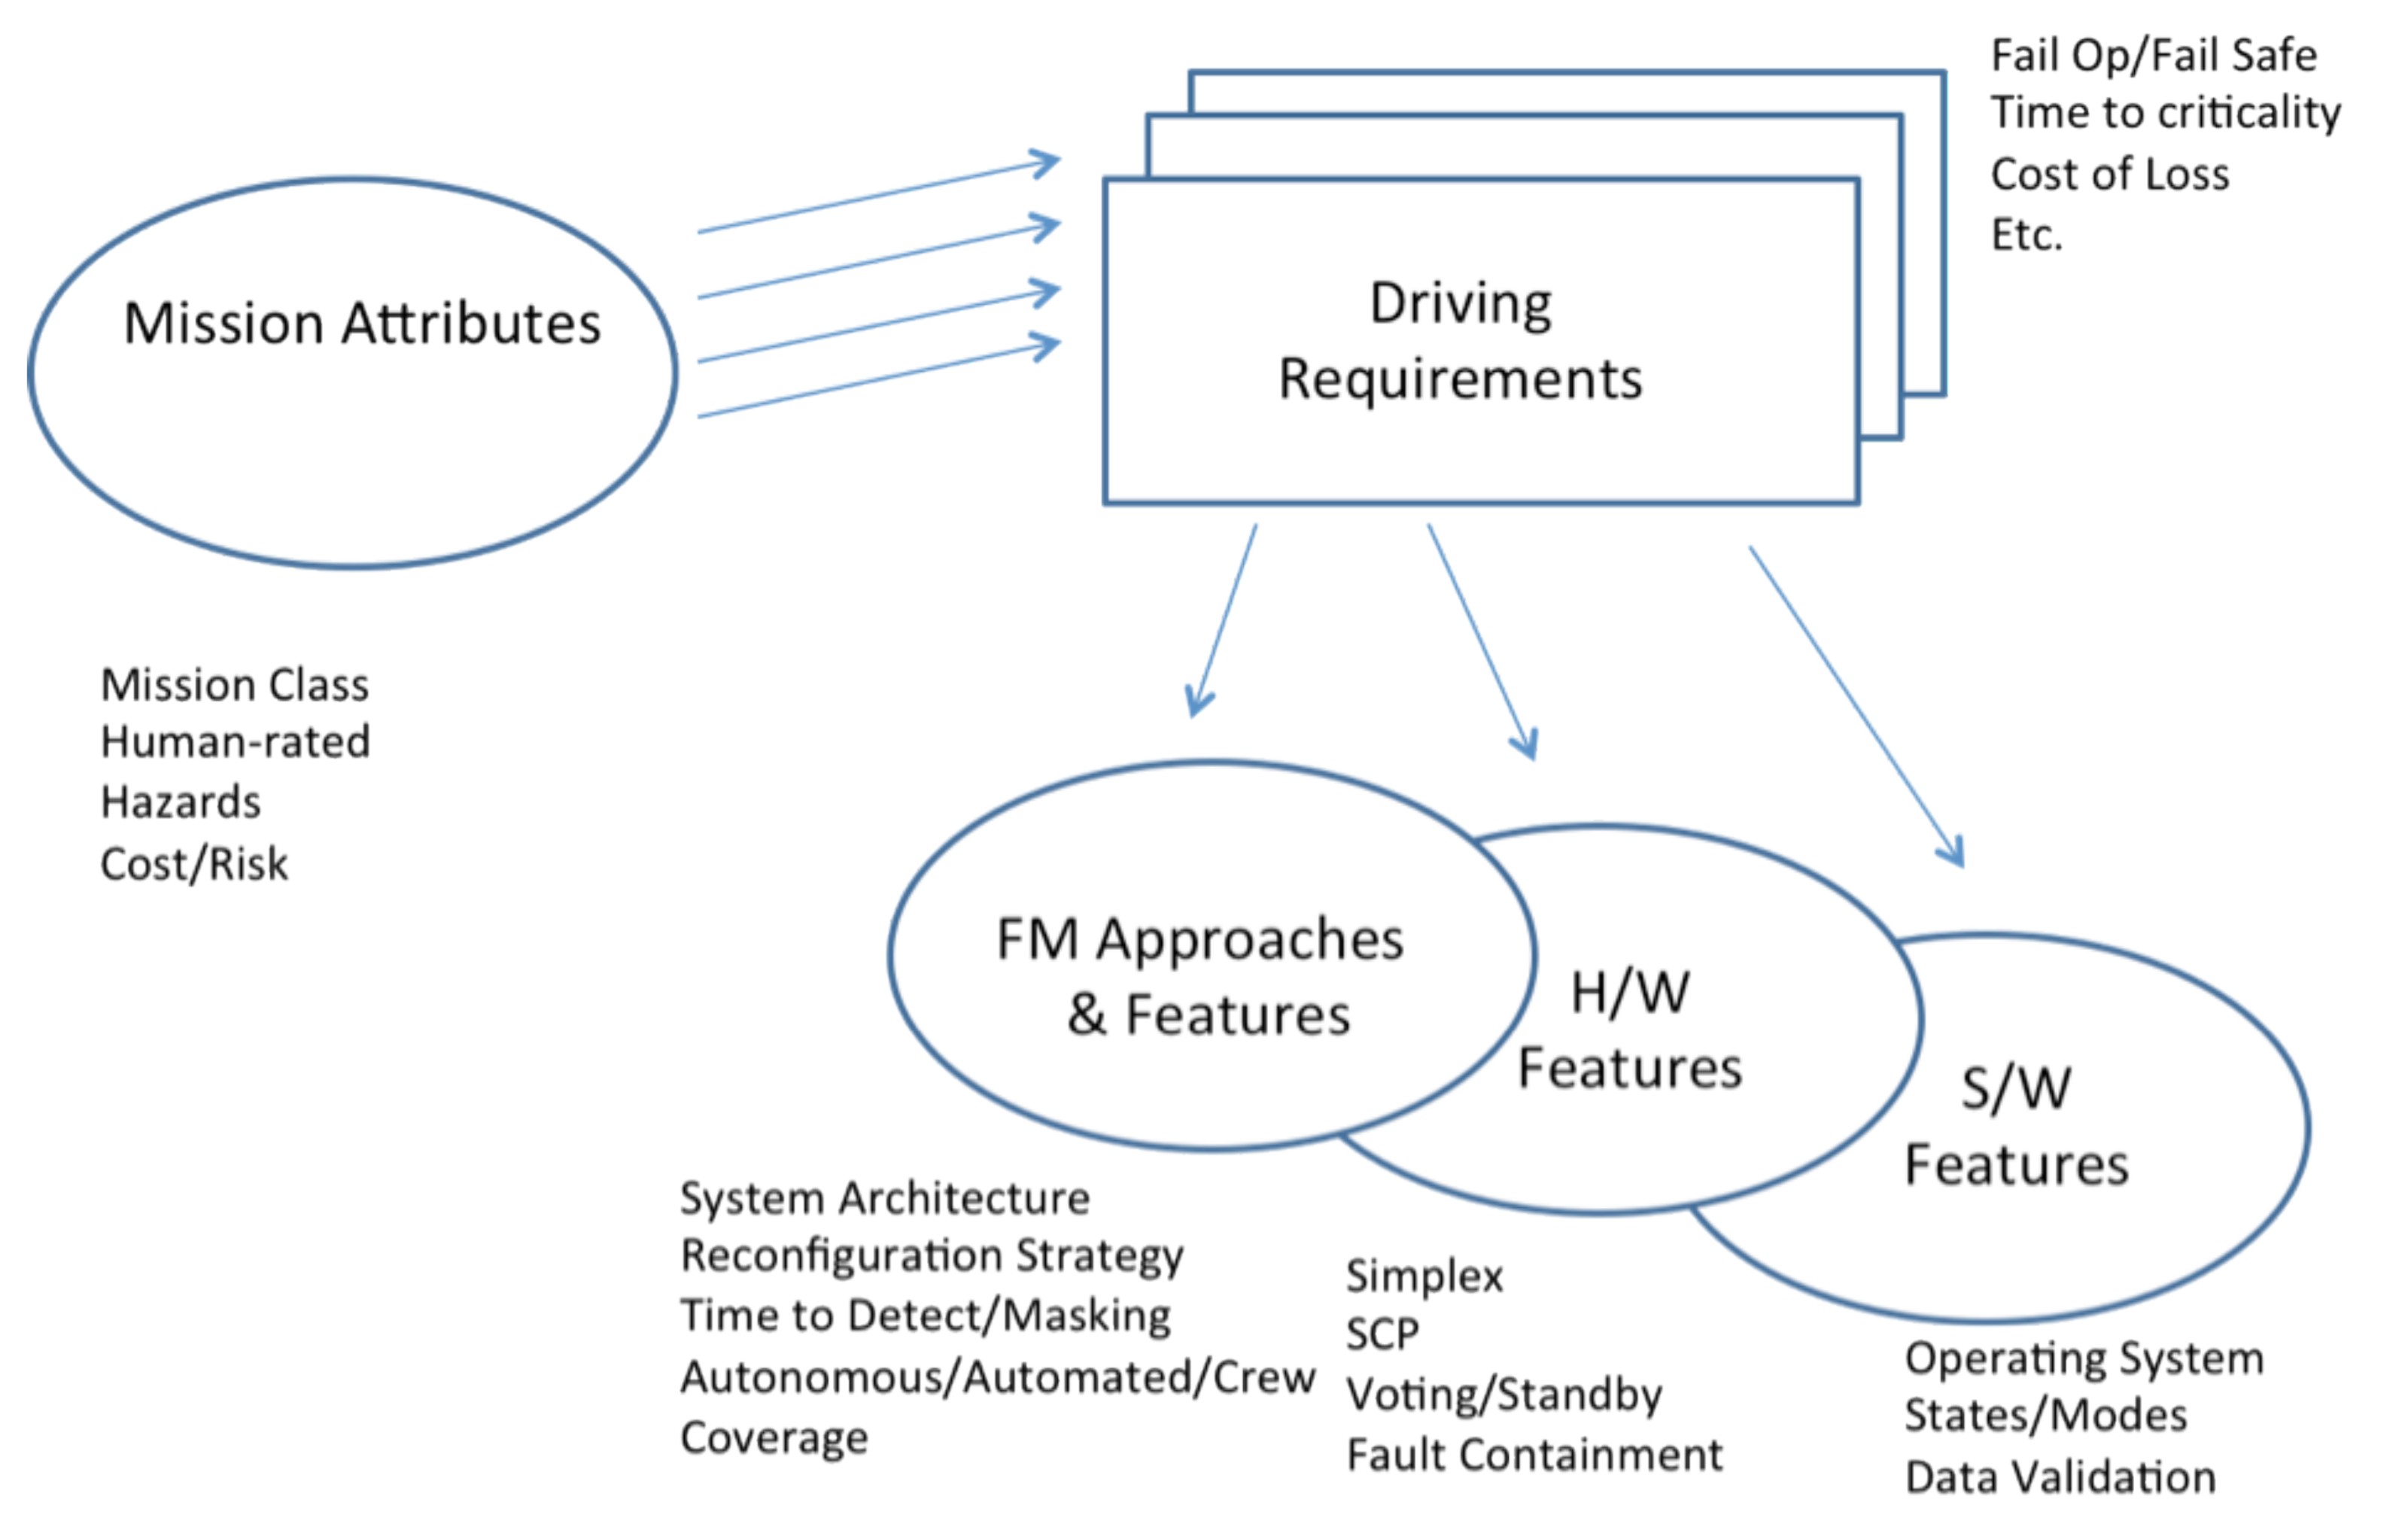
\includegraphics[width=0.8\textwidth]{img/fm_design.png}
	\caption{Fault Management design process. \small{\textit{Source: NASA Fault
	Tolerance Handbook, draft 2, 2012}}}
	\label{fig:fm_design}
	\end{center}
\end{figure}

The first step during development of the FM for a space mission is a clear
identification of mission goals and of functions and resources that are critical
and need to be protected\footnote{These include functions, resources, events
which are needed to achieve the mission's goals. E.g.: successful launch,
scientific payload, collected data etc. }. Subsequently, the FM engineers need
to perform an analysis of the system architecture to identify the mission
characteristics which are definitory for the fault protection functions. Fault
management will need to be implemented throughout the system, however they need
to take into account restrictions enforced by the mission characteristics. For
example, in the case of deep space exploration mission, which have delayed and
infrequent contact with the mission command on Earth, or during time critical
steps of missions (e.g. planetary atmospheric entry), fault management
\textbf{response latency} is critical. According to the NASA Fault Management
Handbook \cite{nasa-fm-handbook}, response latency is \textit{'the time from the
occurrence of a fault to the correction of the failure condition'} and is
\textit{'built from the various mission and system characteristics that impact
the execution of each of the core FM functions'}. To assure system reliability,
the FM response needs to either clear or contain the effects of a failure before
the failure is propagated to other components or before system issues occur.

Over the years, the technologies used for fault protection have been
significantly improved, but the fundamental principals of spacecraft design
have suffered little changes. For example, the fault tolerance design at the
NASA Jet Propulsion Laboratory is based on the following \textbf{fault
management principles} (quoted from \cite{fm-jpl}):
\begin{enumerate}
  \item Respond only to unacceptable conditions
  \item Avoid hair triggers and retriggering
  \item Tolerate false alarms
  \item Make parameters commandable
  \item Corroborate before severe responses
  \item Ensure commandability and long term safety
  \item Preserve consumables and critical data
  \item Log events and actions
\end{enumerate}

The next step followed by the FM engineers is to design and implement software
and hardware solutions to assure the fault protection of a spacecraft. A series
of techniques can be used in different situations and at different moments of
time (different stages). In the presentation of Fault Management at the Jet
Propulsion Lab\cite{fm-jpl}, John Day and Michel Ingham detail a hierarchy of
approaches and give examples of a series of strategies that may be used to
assure fault protection. The hierarchy can be seen in
Figure~\ref{fig:fault_protection_hierarchy}. A first strategy that should be
followed is to to avoid faults altogether, through \textbf{fault avoidance}
techniques. However, for cases when faults do occur, \textbf{fault tolerance}
needs to be in place, to assure that any faults have minimal effects on the ship
and do not cause a mission failure. From this category, for example,
\textbf{Fault Masking}, \textbf{Gradual Degradation} and \textbf{Fault
Detection, Isolation and Recovery} (FDIR) are some general strategies that can
be employed.

\begin{figure}[htb]
	\begin{center}
	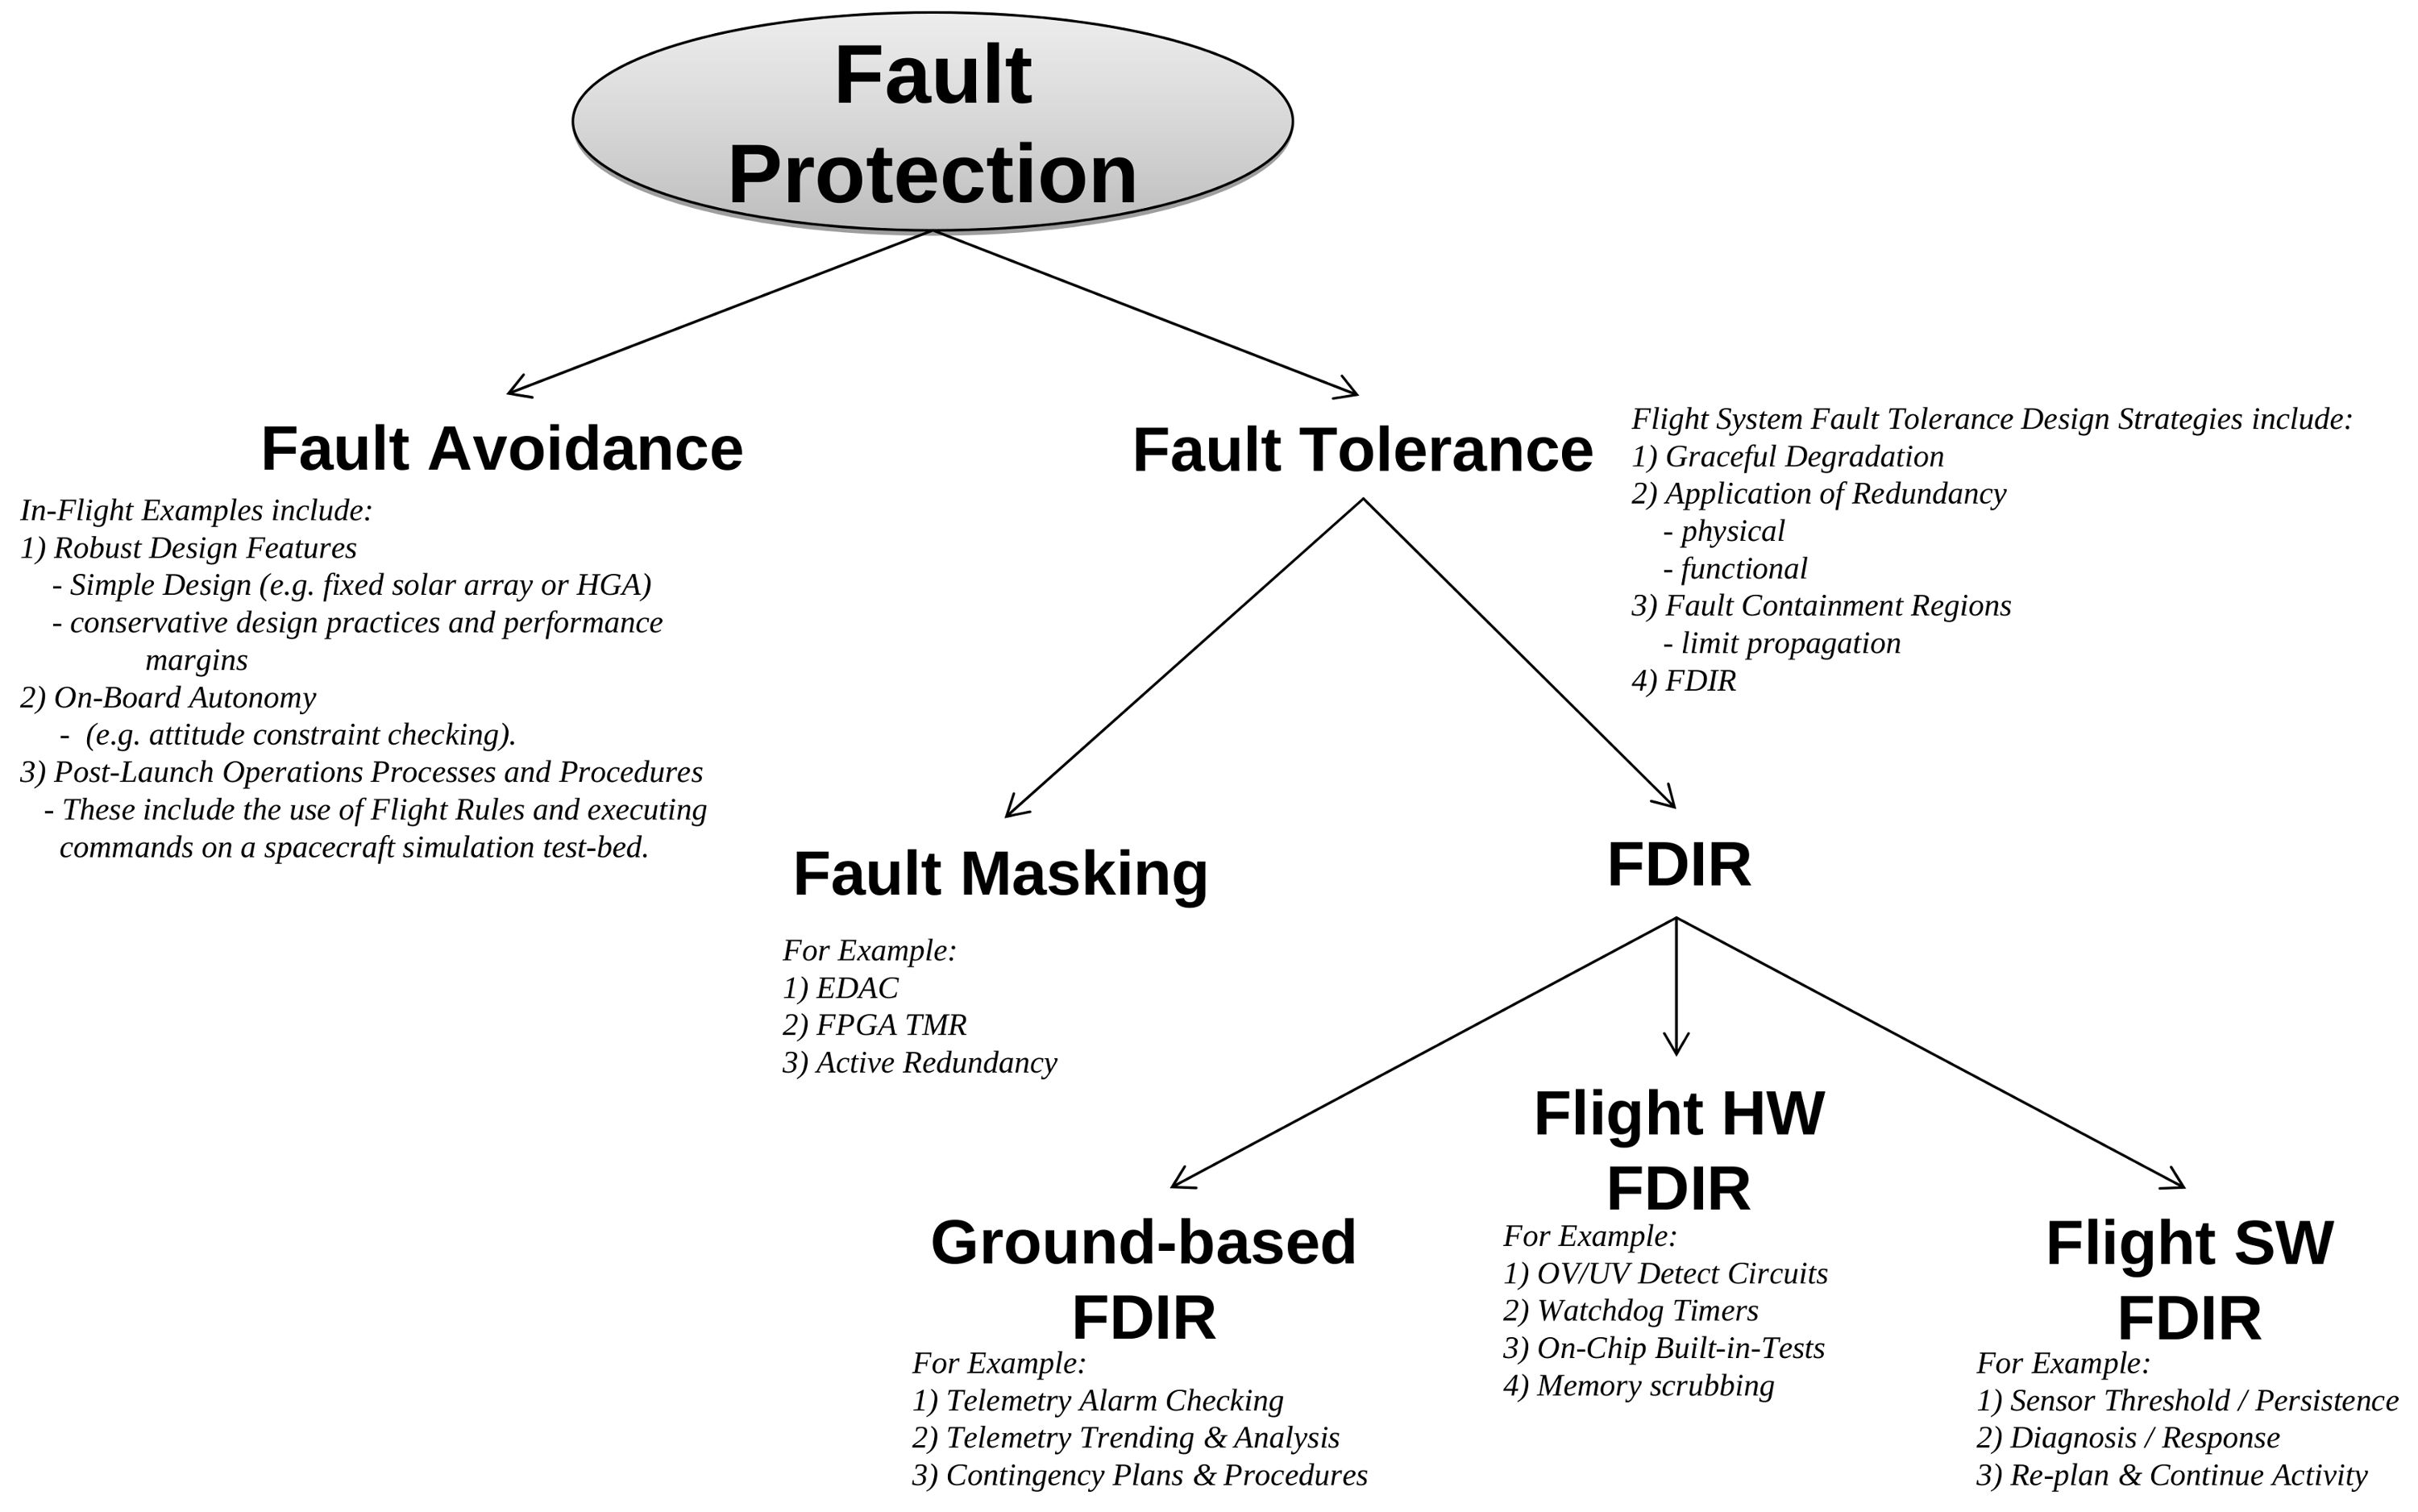
\includegraphics[width=0.9\textwidth]{img/fault_protection_hierarchy.png}
	\caption{Fault protection general hierarchy. \small{\textit{Source: J.
	Day and M. Ingham, Fault management at JPL: past, present and future, 2011}}}
	\label{fig:fault_protection_hierarchy}
	\end{center}
\end{figure}

The design process is one where, mainly because of costs and time restrictions,
usually engineers start from the already developed techniques and technologies
and improve them, increasing the safety, reliability and accuracy. For example,
the most important strategy used for FM is \textbf{Redundancy}. This is usually
implemented in multiple ways\cite{surv-nasa-mars}:
\begin{itemize}
\item Block Redundancy - which ensures that a failure can be solved through the
use of parallel elements
\item Functional Redundancy - which permits the handling of a failure in various
ways
\item Cooperative Redundancy - which permits the division of a system function
in more elements. This helps by allowing the function to be able to succeed despite
the probability of having one of its elements fail
\item Cross Strapping - which permits the system to handle multiple failures
that occur in the system.
\end{itemize}

In the following chapter, we will go into the details of some of the FM
implementations for former NASA deep space exploration missions. However, before
that, a look at the typical execution architecture of spacecrafts is beneficial.
Figure~\ref{fig:spacecraft_execution_architecture} depicts such a generic
architecture, as seen in \cite{fm-jpl}. As it can be observed, command
sequences\footnote{Low-level commands or macros defining actions that need to be
executed for the mission completion.} are being executed by a \textit{nominal
sequencing engine}. Simultaneously, fault protection software is run and is
always prepared to take over the control and execute fault protection actions,
if the behaviours indicate the presence of a fault. Typically, the fault
protection is handled by the Command and Control Subsystem.

\begin{figure}[htb]
	\begin{center}
	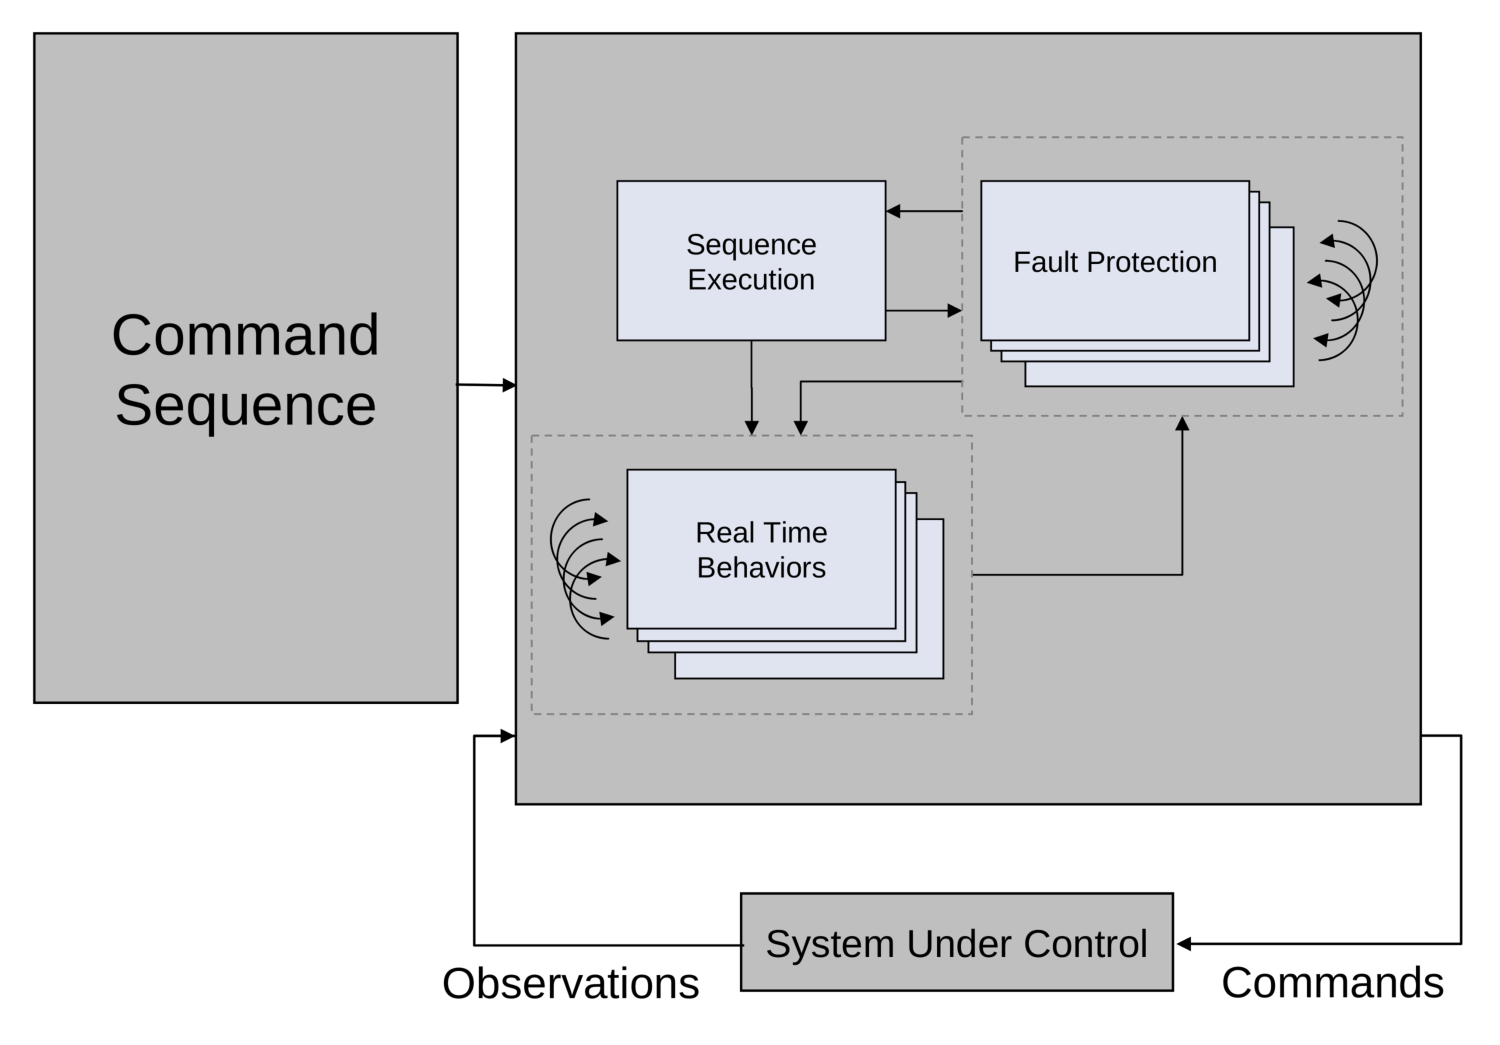
\includegraphics[width=0.6\textwidth]{img/spacecraft_execution_architecture.pdf}
	\caption{Typical Spacecraft Execution Architecture. \small{\textit{Source: J.
	Day and M. Ingham, Fault management at JPL: past, present and future, 2011}}}
	\label{fig:spacecraft_execution_architecture}
	\end{center}
\end{figure}

The design and implementation of FM needs to be followed by Verification and
Validation, to prove that the system complies with the system requirements and
that the response to failures is the intended one. Besides the mission specific
requirements, all space missions have to respect some general safety
requirements. Mandatory ones include the \textbf{NASA General Safety Program
Requirements} (NPR-8715.3) and the \textbf{Eastern and Western Range Safety
Requirements} (EWR 127.1)\footnote{EWR-127.1 represents the specification of
safety requirements for the launch site. It is being replaced with the
\textbf{Air Force Space Command Manual Range Safety User Requirements(AFSCPCMAN
91-710).}}\cite{surv-nasa-mars}. In addition, a multitude of other documents
include recommendations for requirements related to fault protection in the case
of spacecrafts. Some examples include: Rules for the Design, Development,
Verification, and Operation of Flight Systems (GSFC-STD-1000E), NASA Systems
Engineering Processes and Requirements (NPR 7123.1A), Risk Classification for
NASA Payloads (NPR 8705.4) etc.

\section{Case Study - Concrete examples}


\subsection{Voyager}
\subsection{Cassini-Hygens}
\subsection{Mars Climate Orbiter\cite{mco-nasa}}
Mars Climate Orbiter (MCO) was part of the NASA Mars Surveyor program which
included the Mars Global Surveyor as well as Mars Polar Lander. It was launched
in 1998 with the main objective of studying the climate of Mars. It aimed to
monitor atmospheric dust and water vapor as well as taking pictures of the
planet's surface in order to gain insight on the climatic changes. The hope was
to gather evidences that would suport the theory of existing water underneat the
surface of the planet.

MCO was also designed to serve as a communication relay for the Mars Polar
Lander, however after the Lander's mission, it was supposed to conduct its own
main mission independently.

After its nine months jurney to Mars, MCO was lost beacuse it missed its planned
altitude ordbit and fell into the Martian atmosphere where it was distroyed.

The problem identified in the NASA Mishap Investigation Board Phase I
Report~\cite{mco-rep} was that the MCO failed to use metric units in the coding
of a ground software file used in trajectory models. Other causes that contributed to the failure of the
mission included system engineering, traning and organizational factors.

In order to understand better the circumstances that lead to the failure of this
mission, we need to take a closer look at the Attitude Control System and
the fault protection architecture of the MCO~\cite{surv-nasa-mars}.

The MCO's Attitude Control System contained a sun sensor, an inertial
measurement unit, a star camera and reaction wheels. The MCO was controlable in
roll, pitch and yaw so that it can adjust its alttitude, to perform trajectory
maneuvres and to achieve Mars Orbit Inseration. It was designed so that it could
use the gravity force of Mars in order to adjust to the needed velocity which
could allow it to keep the desired orbit and altitude. The design included
rocket engine modules which allowed this as well as serving as elements that
dissipaed any angular momentum which could be accumulated in the reaction
wheels. The Spacecraft Performance Analysis Software (SPAS) was used to
calculate the angular momentum desaturation, however it was not using the
correct units of measures (error in the N to lb-f conversion). This has lead to
the MCO estimating badly its alttitude and orbit.

The fault protection capabilities were unsatisfying at a number of levels in
this mission. First of all, there was an error in the human managemnt process.
The calculation of the automatic momentum desaturation involved a human
constant, because people where involved in loading the information to servers,
also in retrieving it from servers and uploinking it to the MCO. The teams
dealing with the information where not specifically the ones who introduced the
error, however they could have observed the problem and find a solution to
solved it. This proves the existance of a fault in the human-system interaction.
This can be avoided by developing a better system that would allow people to
asses the correctens of the output data based on the input they are giving. It
could be a software solution that would act either as verifier (just calculate
and report the expected results) or as a checker that would identify the
inconcistency and report it.

The critical problem in the MCO case was the lack of an adequate convertor
between the Newtons and lb-f. The software used for the MCO was partly carried
over from another mission (THe Mars Global Surveyor). The privios mission
considered the convertor, however it was not imported for the MCO mission by mistake. The fault could have been
avoided if there would have been thorough testing after the importing of the
already existing software. If the re-used functions would have been inspected
with attention and tests would have been developed in order to check the correct
functionality in the new context, the fault could have been discovered and
solved.

The expectation to have a software system with no bugs or problems is quite
unrealistic. However this should not affect the success of missions. The MCO was
already calculating the angular momentum desaturations and would afterwards
downlinked it to the ground base. At that point the Spacecraft Performance
Analysis Softer was used to calculate the angular momentum desaturation value
without making the correct conversion between Newtons and lb-f. Howver, the
result would be provided to the team in charge and only afterwards the plan for
the future actions would be uplinked to the spacecraft. In this case, another
solution for fault avoidance would have been the limitation or elimination of
the need of the spacecraft to relay on external systems and the human
intervention. Basically, if the the MCO would be designed as to be able to
calculate its own position and only then cross check it with the avilable data
provided by the ground team, it would have been possible to at least notice and
report the problem.

In order to have a good failure tolerance, it was decided that for future
spacecrafts it would be advised to use redundant and independent components
(both software and hardware). In the case of performing the same calculations
with the use of various software modules it could be possible to identify the
differences in the values. In the case of multiple such components, a voting
could be implemented in order to rule out the modules that provide wrong
results.

Since this case is mainly a failure caused by the inadequate re-use of
software, it can be stated that such errors can be avoided through the use of
independent evaluation and validation of the re-used software. The use of
regression testing~\footnote{http://en.wikipedia.org/wiki/Regression\_testing}
as well as comparing results to expected outputs can prove helpful.
\subsection{Mars Reconnaissance Orbiter\cite{mro-nasa}}

The Mars Reconnaissance Orbiter (MRO) was launched on the 12th of August, 2005
and it was one of the first spacecrafts entering Mars' orbit.

Its journey to Mars lasted seven months and it took six more months afterwards
in order for it to reach its science orbit. The MRO was created with the purpose
of tracking changes of the water and dust in Mars' atmosphere. It was also
supposed to look for more evidence of ancient seas and hot springs and to study
the climate changes based on Mars' surface minerals. It also serves as a data
relay station for other missions.

The objectives of the MRO where complex and the probability of failure was high
because of this. There were multiple things that could go wrong with the
mission, considering the complexity of its overall goals and functionality
expectations \cite{mro-mission}.

First of all, the mission was supposed to last about 5.4 years. The system on the spacecraft was supposed
to have an up-time as close as possible to 100\% during this mission. This is
hard to achieve because all possible failures need to be prevented or handled
without losing functionality or precious data.

An analysis of the fault pretection architecture, the effectiveness of this
architecture as well as a categorization of the fault protection capabilities of
the MRO are described in detail in \cite{surv-nasa-mars}.

In order to assure that no big failures cand occur and that, despite its
complexity, the system will work accordingly in order to achieve the mission's
goals, a semi-autonomuos fault protection software (SPIDER - SPacecraft Imbedded
Distributed Error Response) has been developed for the MRO. It has been
developed in C-language with the possibility of re-use for any other future
missions. SPIDER can support redundancy and cross strapping tasks, requirements
which the MRO is supposed to meet.

Despite it's advanced capabilities and the fact that it acts as a first
responder to erros and handles most of them, SPIDER was not design to function
on its own. It still needed help from the ground in order for the system to be
set back in a normal state for the cases when it entered a safe mode. Also,
ground operations where needed in case the system did not recognise some
possibly threatening conditions that could appear. The main advantage of the
SPIDER is that it can actually prevent the system from entering massive failure
without the need to wait for the ground crew to notice and react to the
problems.

FIG - Generic SPIDER Decission process \cite{e-seale}

The SPIDER ensures that the fault responses are general. For example, if the MRO
finds itself in a position in which a fault is detected, than it automatically
switch to a safe mode and interrupt all the uncritical equipment and
functionality. The system can be turned back to normal functionality from the
ground level by the team in charge after following a defined protocol.

The SPIDER ensures that the MRO is not affected by fails at any given time, with
the presumption that only one system can generate failure at a given time. It
basically tries to ensure that the MRO is completely single-fault tolerant and
this leads to the robustness and high relability level of the architecture. As
it was mentioned before, SPIDER was created around the idea of keeping things
redundant and around the cross strapping concept. Among the redundancy technics
it uses we can find:
\begin{itemize}
\item Block Redundancy - which ensures that a failure can be solved through the
use of parallel elements
\item Functional Redundancy - which permits the handling of a failure in various
ways
\item Cooperative Redundancy - which permits the division of a system function
in more elements. This helps by allowing the function to be able to succeed despite
the probability of having one of its elements fail
\end{itemize}

The architechture of the SPIDER is hierarchicle. It has three software levels:
the component level fault protection which is used for communication with the
MRO hardware, the performance level fault protection which keeps track of the
performance of each subsystem and the system level fault protection which tries
to keep failures from happening. Depending on the type of failure, it can be
handled by the befitting logic. In order to avoid starvation, the higher levels
in the hierarchy are allowed to call on to the lower levels in order to assign
them specific tasks, but they cannot take priority of the tasks which
already are executing in these levels.

The SPIDER has been thorughly tested before being integrated on the MRO, but a
final proof of its capability was the fact that, even though the MRO has
encountered quite a few failures during the mission (e.g. memory corruption,
downlink connectivity failure, etc.), it was capable to recover and to achieve
the mission's goals.

\subsection{Mars Exploration Rovers}
\section{Conclusions}
 
\bibliographystyle{abbrv}
\nocite{*}
\bibliography{references}

\end{document}
